\section{Game Design}
\label{sec:game_design}

This chapter covers our game design in regard to game play and the educational aspect.

\subsection{General Concept}
\label{sec:game_design:subsec:general_concept}

Our game design evolves from the idea of a serious game utilizing augmented reality techniques available on larger mobile devices, i.e.\ tablets or phones with a display size of at least 7 inch.
The educational goal is to convey knowledge about Celtic runes and culture through an engaging and entertaining game experience.
Learning is supported by a connection between the matter and the game mechanic, so the player improves his skill in the game by mastering knowledge about runes and vice versa.

The game is designed as a classical Tower Defense (TD) game. Players build towers to defend their city from increasingly difficult hordes of enemies.
This is explained in more detail in Section~\ref{sec:game_design:subsec:tower_defense}.
We use augmented reality to give the player control over the towers and buildings with printed physical markers, our `rune markers' (cf. Section~\ref{sec:game_design:subsec:runes}).
This is meant to increase the learning success by bringing the runes into focus while providing a refreshing game experience through novel control mechanics.
Knowledge about runes and Celtic history is presented gradually using a game campaign, where the player unlocks new runes and additionally information after increasingly more difficult levels. This is thoroughly explained in Section~\ref{sec:game_design:subsec:campaign}.

Finally we based the style of the game on available historical data about Celtic cities, defenses and enemies, which is covered in Section~\ref{sec:game_design:subsec:history}.

\subsection{Runes and Rune Markers}
\label{sec:game_design:subsec:runes}

As the primary goal of playing the game is to learn about Celtic runes, the runes are the core of our game experience.
Therefore we split the game into two distinct phases:
A preparation phase where the player interacts with physical representations of the runes, our rune markers, and a game phase where the player interacts with the augmented reality device.

\begin{wrapfigure}{R}{0.38\textwidth}
	\centering
	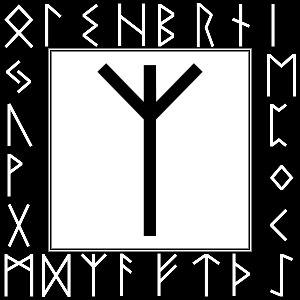
\includegraphics[width=0.35\textwidth]{figures/algiz0.jpeg}
	\caption{\label{fig:rune-marker} An Algiz rune marker for building towers}
\end{wrapfigure}

Our rune markers are printed out representations of runes that each have a unique effect in the game and need to be properly positioned by the player. Figure~\ref{fig:rune-marker} shows a rune marker for the \textit{`Algiz'} rune, which is used to build and position towers in-game.
As a player can use some runes multiple times, the rune markers have an additional unique boarder that enables the augmented reality tracking to distinguish similar runes.

As the basis for our runes and rune markers we used the 24 runes of the \textit{`Elder Futhark'}~\cite{elder-futhark}, the oldest form of the runic alphabets.
Almost\footnotemark all of the 24 runes have a special meaning in the game that closely relates to their original meaning.
For example the Algiz rune has the meanings \textit{`Elk', `Protection', `Defense'}~\cite{algiz} and is used to build towers.
Though, it must be noted here though that runes can have multiple meanings and the meaning is not always absolutely clear.
Rieckhoff and Biel point out that there is not Celtic historiography, literature or religious writings.~\cite{rieckhoff-runes} The absence of a large basis of usage, makes interpreting runes especially difficult.
\footnotetext{Unfortunately, we had to skip some runes as there was no reasonable way of mapping the rune to an in-game functionality.}
A complete table of the runes we used, the original meaning we used as a basis and their usage in-game can be found in Appendix~\ref{appendix-a}.

To properly play the game a player must recognize a rune and it's function in-game.
The player has as much time as he needs to study, recognize and properly place the runes in the preparation phase.\footnotemark
In combination with the coverage of most runes in-game and a close relation of their traditional meaning to the in-game usage, this measures support the learning success of the player.

\footnotetext{Though this can help him learn the runes, this was also a necessity due to the nature of augmented reality on a tablet computer.}

\subsection{Tower Defense}
\label{sec:game_design:subsec:tower_defense}

We use the basic and popular tower defense concepts for our core gameplay mechanics. Towers are manually placed on the map (through the position of the rune markers relative to the augmented reality map) and shoot incoming waves of enemies. The enemies have to be killed before they can reach the village, which is positioned with the \textit{`Mannaz'} rune marker and the anchor point of the augmented reality map.
If enemies reach the village, players loose health. When health reaches zero, the game is lost and the player has to start over.

Players can upgrade their towers by placing buff runes close to their tower rune. For example the \textit{`Kenaz'} rune adds fire damage to the tower it's linked to.
As enemies are vulnerable to different damage types, e.g. a wooden siege weapon is vulnerable to fire damage, players have to carefully consider their elemental upgrades.
Additionally players can earn gold by building farms and harvesting them during the game phase, which adds additional interactivity to the game phase.
The gold can be used to buy additional lives during the preparation phase.

Although, we would've liked to implement advanced mechanics we decided to stick with this basic tower defense principles, which works with our augmented reality setup and is intuitive to use, because of the difficulties encountered (cf. Section~\ref{sec:problems}).


\subsection{Campaign}
\label{sec:game_design:subsec:campaign}

The game and also the learning process is structured into increasingly difficult levels. At each level the player unlocks new runes, gets information about the runes historical meaning and it's use in-game.
E.g. in the first level the player unlocks the \textit{`Mannaz'} and \textit{`Algiz'} rune so he can build the village and his first tower. In the second level he unlocks another \textit{`Algiz'} rune for a second tower and a \textit{`Jera'} rune to build a farm he can harvest during the game phase.
The player gets textual information in a dialog window and an enlarged image of the new rune.
He has to immediately learn to recognize the rune to be able to find the rune marker with the rune and use it to construct or enhance buildings.
For additional references the player can open a \textit{`wiki'}, where he can find all information about runes and the game in a structured format.
We chose this structured campaign approach, because we quickly realized while testing that 24 runes with different meanings is overwhelming when directly available and a slower introduction in small manageable steps yields better results.

Each level also spawns new and tougher enemies, so the player is forced to use his runes wisely to beat the level and advance in the campaign.
After beating the campaign, a free-play mode is unlocked to offer a challenge with all runes available.


\subsection{Historical Reference}
\label{sec:game_design:subsec:history}

We created a mostly historical accurate setting for the game. Because we used a self-made voxel engine (cf. Section~\ref{sec:implementation:voxelframework} to render our game, we were able to create the game assets by ourselves.

Our Celtic village is based on reconstructions of the \textit{`Oppidum of Manching'} as illustrated in~\cite{kraemer-oppidum-maching}. The tower and stone walls were modeled after historically funded illustrations from~\cite{kraemer-oppidum-maching}\cite{rieckhoff-walls1}\cite{rieckhoff-walls2}\cite{rieckhoff-tower}. A selection of these illustrations can be found in Appendix~\ref{appendix-b}. As enemies we created attackers that the Celts may have actually encountered.
They get attacked by wolves and bears in the beginning and later by invading Roman foot soldiers and siege weapons.
The attackers may also be accompanied by mythical creatures the Celts believed in like the Kelpie, a equine water spirit.

Figure~\ref{fig:house-comparison} shows a comparison between our house asset and the illustrated reconstruction from Manching as found in~\cite{kraemer-oppidum-maching}.
Though we had to make the house a little bit taller, because the angles for the roof that look good are limited by the voxel design.

\begin{figure}[ht]
	\centering
	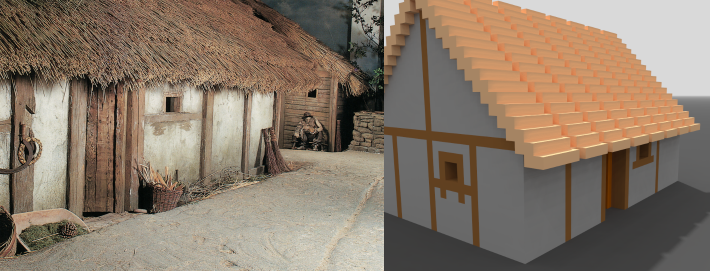
\includegraphics[width=\linewidth]{figures/house_comparison.png}
	\caption{Our house design compared with an illustration from Manching.}
	\label{fig:house-comparison}
\end{figure}







